\section{Modelo de información del sistema}
En la Figura \ref{fig:Base_ServidorEmbebido} se observa un diagrama del modelo de información correspondiente al servidor embebido, se puede observar que las tablas no se encuentran relacionadas, esto es debido a que la información que almacenan no está ligada de ninguna forma con el resto, a pesar de que los registros de algunas tablas sirvan para calcular los registros de otras.
\begin{figure}[H]
	\centering
	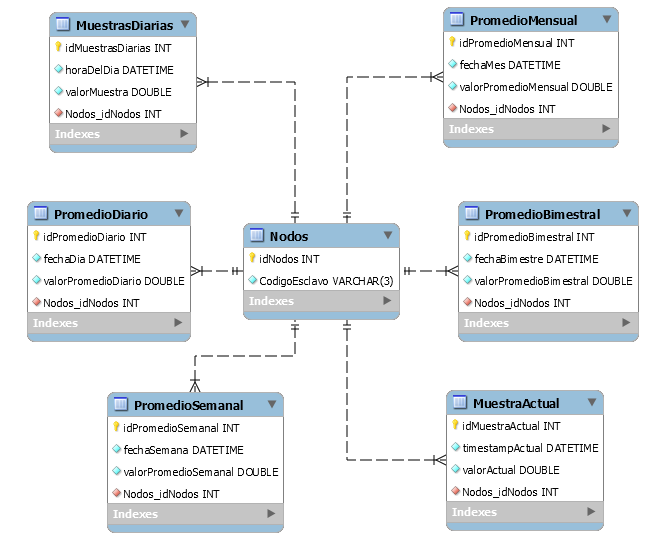
\includegraphics[scale=1.26]{Capitulo4/images/Base_ServidorEmbebido.PNG}
	\caption{Modelo de información del Servidor Embebido}
	\label{fig:Base_ServidorEmbebido}
\end{figure}

A continuación en la Figura \ref{fig:Base_AplicacionUsuario} se muestra el diagrama del modelo de información correspondiente a la aplicación de usuario, en donde se puede observar que únicamente se almacenará en la aplicación las notificaciones y los servidores que den respuesta a las peticiones de la aplicación de usuario, la relación entre tablas nos indica que muchas notificaciones pueden pertenecer a un mismo servidor.

\begin{figure}[H]
	\centering
	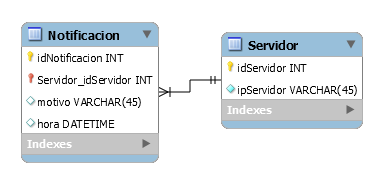
\includegraphics[scale=1.26]{Capitulo4/images/Base_AplicacionUsuario.PNG}
	\caption{Modelo de información de la aplicación de usuario}
	\label{fig:Base_AplicacionUsuario}
\end{figure}